\documentclass[tikz,border=7pt]{standalone}
\usetikzlibrary{matrix,fit,positioning, arrows.meta,
  decorations.pathreplacing, calc}
\begin{document}
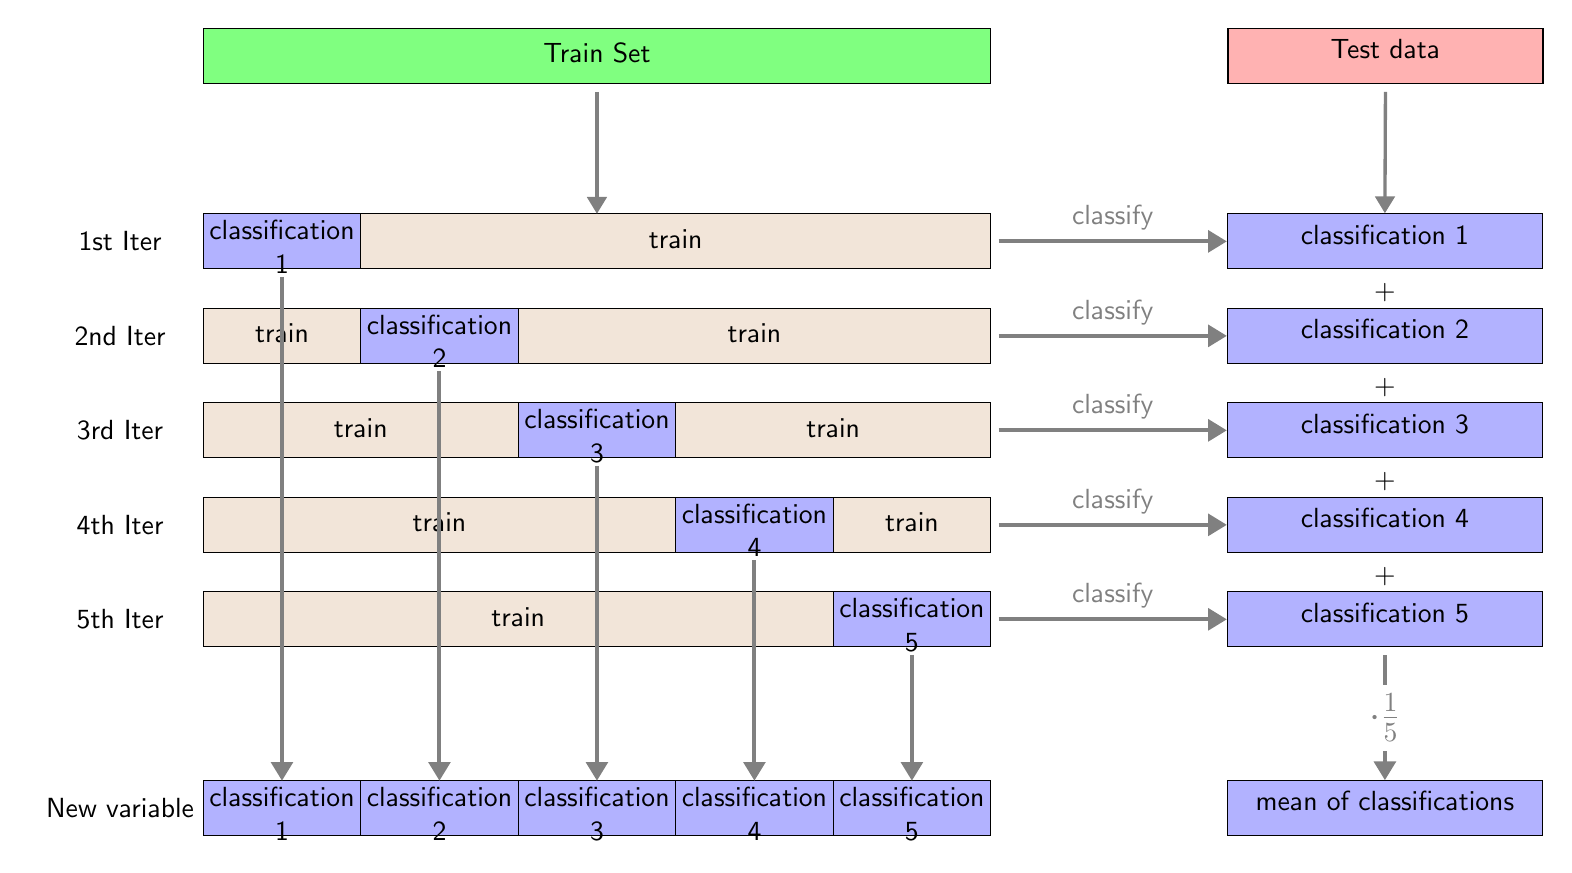
\begin{tikzpicture}[font=\sffamily,
  standard/.style={inner sep=0pt,align=center,draw,%text
    % height=1.25em,
    minimum height = 7mm,
    text depth=0.5em},
  decoration={brace},
  oneblock/.style={transform shape,minimum width=1cm,draw},
  zusatz/.style={draw=green!30, anchor=south west, minimum
    width=2cm,minimum height=7mm}]
    \matrix (M) [
        matrix of nodes,
        nodes={
%          text height=1.25em,
%          text depth=2cm,
            minimum height = 7mm,
            minimum width = 2cm,
            outer sep=0,
           anchor=center,
           fill=brown!20 % <-added
        },
        column 1/.style={
            nodes={draw=none,fill=none}, % <-- added fill=none
            minimum width = 4cm
          },
        column 7/.style={
            nodes={draw=none,fill=none,align=left}, % <-- added fill=none
            minimum width = 4cm
        },
        row sep=5mm, column sep = 0,%column sep=-\pgflinewidth,
        nodes in empty cells,
        e/.style={fill=blue!30},
        alignleft/.style={draw=none, fill=none,align=left}
      ]
      {
        1st Iter & |[e]| & & & & &|[draw=none, fill=none]|\\
        2nd Iter & & |[e]| & & & &|[draw=none, fill=none]| \\
        3rd Iter & & & |[e]| & & &|[draw=none, fill=none]| \\
        4th Iter & & & & |[e]| & &|[draw=none, fill=none]| \\        
        5th Iter & & & & & |[e]| &|[draw=none, fill=none]|\\
        |[draw=none,fill=none]| &|[draw=none, fill=none]|
        &|[draw=none, fill=none]| & |[draw=none,
        fill=none]|&|[draw=none, fill=none]| &|[draw=none, fill=none]| &|[draw=none, fill=none]|\\
        New variable & |[e]|& |[e]|& |[e]|&
        |[e]|&|[e]| &\\
      };
      \node[fit=(M-1-3) (M-1-6), standard,fill=none, draw]{train};
      \node[fit=(M-1-2) (M-1-2), standard, fill=none, draw]{classification 1};
      \node[fit=(M-2-2) (M-2-2), standard, fill=none, draw]{train};
      \node[fit=(M-2-3) (M-2-3), standard, fill=none, draw]{classification 2};
      \node[fit=(M-2-4) (M-2-6), standard, fill=none, draw]{train};
      \node[fit=(M-3-2) (M-3-3), standard, fill=none, draw]{train};
      \node[fit=(M-3-4) (M-3-4), standard, fill=none, draw]{classification 3};
      \node[fit=(M-3-5) (M-3-6), standard, fill=none, draw]{train};
      \node[fit=(M-4-2) (M-4-4), standard, fill=none, draw]{train};
      \node[fit=(M-4-5) (M-4-5), standard, fill=none, draw]{classification 4};
      \node[fit=(M-4-6) (M-4-6), standard, fill=none, draw]{train};
      \node[fit=(M-5-2) (M-5-5), standard, fill=none, draw]{train};
      \node[fit=(M-5-6) (M-5-6), standard, fill=none, draw]{classification 5};
      \node[fit=(M-7-2) (M-7-2), standard, fill=none, draw]{classification 1};
      \node[fit=(M-7-3) (M-7-3), standard, fill=none, draw]{classification 2};
      \node[fit=(M-7-4) (M-7-4), standard, fill=none, draw]{classification 3};
      \node[fit=(M-7-5) (M-7-5), standard, fill=none, draw]{classification 4};
      \node[fit=(M-7-6) (M-7-6), standard, fill=none, draw]{classification 5};                  
       \node[fit=(M-1-2) (M-1-6), fill=green!50,
       yshift=2cm, standard, anchor=south](trs) {Train Set};
       \draw[->][black!50, line
       width=1.2pt,-Triangle](trs.south) ++(0,-1mm)-- (M-1-4.north);
        \node[right=3cm of trs,standard,fill=red!30,text width=4cm,
        anchor=west] (tes) {Test data};
        \node[right=3cm of M-1-6,standard,fill=blue!30,text width=4cm,
        anchor=west] (tes1) {classification 1};
        \node[right=3cm of M-2-6,standard,fill=blue!30,text width=4cm,
        anchor=west] (tes2) {classification 2};
        \node[right=3cm of M-3-6,standard,fill=blue!30,text width=4cm,
        anchor=west] (tes3) {classification 3};
        \node[right=3cm of M-4-6,standard,fill=blue!30,text width=4cm,
        anchor=west] (tes4) {classification 4};
        \node[right=3cm of M-5-6,standard,fill=blue!30,text width=4cm,
        anchor=west] (tes5) {classification 5};
        \node[right=3cm of M-7-6,standard,fill=blue!30,text width=4cm,
        anchor=west] (tes7) {mean of classifications};
        \node [below=1.5pt] at (tes1.south) {$+$};
        \node [below=1.5pt] at (tes2.south) {$+$};
        \node [below=1.5pt] at (tes3.south) {$+$};
        \node [below=1.5pt] at (tes4.south) {$+$};
        \draw[->][black!50, line width=0.5mm, -Triangle] (tes5.south)
        ++(0,-1mm)-- (tes7.north) node[midway, fill=white]{\Large
          $\cdot \frac{1}{5}$};
        \draw[->][black!50, line
       width=1.2pt,-Triangle](tes.south) ++(0,-1mm)-- (tes1.north);
       % \node[oneblock, minimum height = 7mm, minimum width = 2cm,
       % anchor=west,right=of M-2-6,fill=brown!20,outer sep=0mm] (A1)
       % {Train};
       % \node[oneblock, minimum height = 7mm, minimum width = 2cm,
       % anchor=east,right=of M-3-6,fill=blue!30,outer sep=0mm] (A2) {Test};       
      % fold labels and arrows
       \foreach [
             count=\row,
             evaluate={\col=ifthenelse(\row==99, % if fourth row
                                       int(\row+3), % use seventh column
                                       int(\row+1)) % else use column row+1
                       }
                ] \txt in {1,2,3,4,5}
         {
           \draw[->][black!50, line
           width=0.5mm,-Triangle](M-\row-\col.south) ++(0mm,-1mm) --
           (M-7-\col.north);
           \draw[->][black!50, line width=0.5mm, -Triangle]
           (M-\row-6.east) ++(1mm,0) -- (tes\row.west) node[midway,above]{classify};
          }

  \end{tikzpicture}
\end{document}
%%% Local Variables:
%%% mode: latex
%%% TeX-master: t
%%% End:

